\chapter{Large-Scale Kernel Methods for Unstructured Datasets}
\label{chap:unstructured_datasets}
In vast majority of real-world problems the data sets do not have the factorial structure.
In this case the are several approaches to scale up the GP model.
One way is to aggregate several smaller models into big one,
e.g. Mixture of GPs and Bayesian Machine Committee
\citep{rasmussen2006gaussian, rasmussen2001infinite}.
The idea here is to split data set into several smaller subsets
$\mathcal{D}_i, i=1, \ldots, M$, build on each data set GP model and then combine them.
In Bayesian committee machine, for example, the final distribution is given by
\[
    p(y^* | \mathcal{D}) \sim \frac{\prod_{i=1}^M p(y^* | \mathcal{D}_i)}{p(y^*)},
\]
supposeing that the correlation between subsets is small.

Another class of methods builds lightweight approximation of the kernel function.
There are data dependent approaches that follow Nystr{\"o}m's method for kernel approximation
\citep{rasmussen2006gaussian}.
The idea of approximation is based on numerical approximation of the {\em eigenfunctions}
and {\em eigenvalues} of the kernel function.
A function $\phi(\cdot)$ that satisfies the following equation
\[
    \int k(\mathbf{x, x}')\phi(\mathbf{x}) d\mu(\mathbf{x}) = \lambda \phi(\mathbf{x}')
\]
is called eigenfunction of kernel $k$, $\lambda$ is a corresponding eigenvalue
with respect to measure $\mu$.
If we let $d\mu(\mathbf{x}) = p(\mathbf{x})d\mathbf{x}$ we can write down
numerical approximation to the equation
\begin{equation}
\label{eq:eigenfunction_approx}
    \lambda_i \phi_i(\mathbf{x}) \simeq
    \frac{1}{M} \sum_{k=1}^M k(\mathbf{x}_k, \mathbf{x}) \phi_i(\mathbf{x}_k),
\end{equation}
where points $\mathbf{x}_k$ are generated from distribution $p(\mathbf{x})$
and called {\em inducing points}.
By plugging $\mathbf{x}_i$ from the training set into equation above we obtain
\[
    \mathbf{K}_f \mathbf{u}_i = \hat{\lambda}_i \mathbf{u}_i,
    \quad
    \phi_i(\mathbf{x}_j) = \sqrt{\hat{\lambda}_i} \left ( \mathbf{u}_i \right )_j.
\]
And now from \eqref{eq:eigenfunction_approx} we obtain {\em Nystr{\"o}m} approximation
of the $i$-th eigenfunction $\phi(\mathbf{x}) = \frac{M}{\hat{\lambda}_i}\mathbf{k}^\T \mathbf{u}_i$, and, therefore, approximation of the kernel matrix
\begin{equation}
\label{eq:nystrom_matrix}
    \mathbf{K}_f \simeq \widehat{\mathbf{K}}_f = \mathbf{K}_{NM}\mathbf{K}_{MM}^{-1}\mathbf{K}_{MN},
\end{equation}
where $\mathbf{K}_{MN}$ is a covariance matrix between training points and inducing points
and $\mathbf{K}_{MM}$ is a covariance between inducing points.
More details can be found in \citep{rasmussen2006gaussian}.

In \citep{williams2001using} the authors first proposed to use
\eqref{eq:nystrom_matrix} approximation in posterior distribution of GP regression model.
The computational complexity is reduced to $\mathcal{O}(NM^2 + M^3)$ operations
which gives benefit if $M \ll N$.
There are several works that build on top of Nystr{\"o}m approximation trying to refine
the approximation of the covariance matrix and, thus, improve the quality of the model
while preserving low computational complexity \citep{quinonero2005unifying, rossi2020sparse}.

In this thesis we consider different type of approximations based on so called
{\em random features}.
The idea of the approach is to construct approximation of the kernel function
that enables low-rank approximation of the kernel matrix.
To construct such approximation we need to consider the kernel function from different
perspective.
It turns out that every positive definite kernel $k$ uniquely defines some space of functions
and vice versa.
Moreover, it can be seen as an inner products in an appropriate Hilbert space.

\begin{definition}[Positive definite kernels]
    Let $\mathcal{X}$ be a nonempty set.
    A symmetric function $k \colon \mathcal{X} \times \mathcal{X} \rightarrow \mathbb{R}$
    is called a positive definite kernel, if for any set $\mathbf{x}_1, \ldots, \mathbf{x}_N$,
    $\forall N \in \mathbb{N}$ and for any $(c_1, \ldots, c_N)\subset \mathbb{R}$ it holds
    \[
        \sum_{i=1}^N \sum_{j=1}^N c_i c_j k(\mathbf{x}_i, \mathbf{x}_j) \geq 0.
    \]
\end{definition}

Note, that the covariance function that we use in GP are also positive definite kernels.

\begin{definition}[RKHS, \citep{aronszajn1950theory}]
Let $\mathcal{X}$ be a nonempty set and $k$ be a positive definite kernel on $\mathcal{X}$.
A Hilbert space $\mathcal{H}$ of function on $\mathcal{X}$ with an inner-product
$\langle \cdot, \cdot \rangle_{\mathcal{H}}$ is called a reproducing kernel
Hilbert space (RKHS) with reproducing kernel $k$, if the following is satisfied
    \begin{enumerate}
        \item For all $\mathbf{x} \in \mathcal{X}$ we have
        $k(\cdot, \mathbf{x}) \in \mathcal{H}$;
        \item for all $\mathbf{x} \in \mathcal{X}$ and for all $f\in \mathcal{H}$
        \[
            f(\mathbf{x}) = \langle f, k(\cdot, \mathbf{x}) \rangle
            \tag*{Reproducing property}.
        \]
    \end{enumerate}
\end{definition}
In reproducing property we used $k(\cdot, \mathbf{x})$ which is actually
a real-valued function such that $\mathbf{y} \rightarrow k(\mathbf{y, x})$
for $\forall \mathbf{y} \in \mathcal{X}$.
So, the kernel function satisfies
\[
    k(\mathbf{x, y}) = \langle k(\cdot, \mathbf{x}), k(\cdot, \mathbf{y}) \rangle,
    \quad \mathbf{x, y} \in \mathcal{X}.
\]
$k(\cdot, \mathbf{x})$ is called {\em canonical feature map} of $\mathbf{x}$.
There can be a lot of different features maps
$\psi \colon \mathcal{X} \rightarrow \mathcal{H}$ such that their inner product is defined
by the kernel function $k(\mathbf{x, y}) = \langle \psi(\mathbf{x}), \psi(\mathbf{y})$.

The idea for kernel approximation using randomized feature map is based
on finding finite-dimensional maps that approximate the inner-product that is associated
with the kernel function.

The main contributions of this chapter are as follows.
\begin{itemize}
    \item We introduce a technique for kernel approximation based on randomzied feature maps
    and special quadrature rules.
    \item We derive error bounds for the developed approach.
    \item We show that \citep{rahimi2008random,felix2016orthogonal} are special cases of the
    proposed method.
\end{itemize}




\section{Quadrature-based Features for Kernel Approximation}

\subsection{Random Fourier Features}
\label{sec:random_fourier_features}
One of the most well-known approach is called
Random Fourier Features (RFF).
It was first proposed by \citep{rahimi2008random}, and it is based on Bochner's theorem.
\begin{theorem}[Bochner]
    A continuous kernel $k(\mathbf{x, x'}) = k(\mathbf{r}), \mathbf{r = x - x'}$ on
    $\mathbb{R}^d$ is positive definite if and only if
    $k(\mathbf{r})$ is a Fourier transform of a non-negative measure $p(\mathbf{w})$
    \begin{equation}
    \label{eq:bochner}
        k(\mathbf{r}) = \int_{\Omega} p(\mathbf{w}) e^{j\mathbf{w^{\T}(x - x')}} d\mathbf{w}.
    \end{equation}
\end{theorem}
By applying Monte-Carlo sampling to approximate integral in~\eqref{eq:bochner}
RFF introduces a low-dimensional randomized approximation to feature maps:
\begin{equation}
\label{eq:inner}
    k(\mathbf{x, y}) \approx
    \mathbf{\hat{\Psi}}(\mathbf{x})^{\boldsymbol{\top}} \mathbf{\hat{\Psi}}(\mathbf{y}),
\end{equation}
\[
    \mathbf{\hat{\Psi}}(\mathbf{x}) =
    \frac{1}{\sqrt{D}} \begin{bmatrix}
        \cos(\mathbf{w}_1^\T\mathbf{x}) \\
        \sin(\mathbf{w}_1^\T \mathbf{x}) \\
        \cdots \\
        \cos(\mathbf{w}_D^\T \mathbf{x}) \\
        \sin(\mathbf{w}_D^\T \mathbf{x}) \\
    \end{bmatrix}, \quad \mathbf{w}_i \sim p(\mathbf{w}),
\]
where $D$ is a number of generated samples.
Exploiting the idea with an integral representation of the dot product
\[
k(\mathbf{x, y}) = \int_{\Omega} \psi(\mathbf{w, x}) \psi(\mathbf{w, y}) p(\mathbf{w}) d\mathbf{w},
\]
we can construct low-rank approximations to a wider class of kernel functions
(not only shift-invariant kernels).
In this case the feature map $\mathbf{\hat{\Psi}}(\mathbf{x})$ looks like
\[
    \mathbf{\hat{\Psi}}(\mathbf{x}) = \frac{1}{\sqrt{D}} \begin{bmatrix}
        \psi(\mathbf{w}_1, \mathbf{x}) \\
        \cdots \\
        \psi(\mathbf{w}_D, \mathbf{x})
    \end{bmatrix},
    \quad
    \mathbf{w} \sim p(\mathbf{w}).
\]








A randomized $D$-dimensional mapping $\mathbf{\hat{\Psi}}(\cdot)$ applied to the original data
input allows employing standard linear methods, i.e. reverting the kernel trick. In doing so
one reduces the complexity to that of linear methods, e.g. $D$-dimensional approximation
admits $\mathcal{O}(ND^2)$ training time, $\mathcal{O}(ND)$ memory and  $\mathcal{O}(N)$
prediction time.

It is well known from the theory on Monte Carlo based estimates
that as $D \rightarrow \infty$, the randomized feature maps based
approximations converge to the exact kernel $k(\mathbf{x, y})$.
Recent research \citep{yang2014quasi, felix2016orthogonal, choromanski2016recycling} aims to improve the convergence of approximation so that a smaller $D$ can be used to obtain the same quality of approximation.

Here we will consider the class of kernels admitting the following integral representation
\begin{equation}
\label{eq:integral_representation}
    \begin{aligned}
        k(\mathbf{x}, \mathbf{y}) =
        \mathbb{E}_{p(\mathbf{w})} f_{\mathbf{xy}}(\mathbf{w}) =
        I(f_{\mathbf{xy}}),
        \quad p(\mathbf{w}) = \frac{1}{(2 \pi)^{d/2}} e^{-\frac{\|\mathbf{w}\|^2}{2}},
        \\
        \quad f_{\mathbf{xy}} = \phi(\mathbf{w}^{\T}\mathbf{x})
        \phi(\mathbf{w}^{\T} \mathbf{y}).
    \end{aligned}
\end{equation}
It includes the class of shift-invariant kernels,
e.g. the popular Gaussian kernel with
$f_{\mathbf{xy}}(\mathbf{w}) =
\phi(\mathbf{w}^{\boldsymbol{\top}}\mathbf{x})^{\boldsymbol{\top}}
\phi(\mathbf{w}^{\boldsymbol{\top}}\mathbf{y})$,
where $\phi(\cdot) = \begin{bmatrix}\cos(\cdot) & \sin(\cdot) \end{bmatrix}^{\boldsymbol{\top}}$.
It also contains Pointwise Nonlinear Gaussian (PNG) kernels.
They are widely used in practice and have interesting connections with neural networks
\citep{cho2009kernel, williams1997computing}.

The main challenge for the construction of low-dimensional feature maps is the approximation of the expectation in \eqref{eq:integral_representation} which is $d$-dimensional integral with Gaussian weight.
To improve the approximation we introduce quarature rules to approximate the integral
and then show that they generalize several prominent papers in this topic.
% Unlike other research studies we refrain from using simple Monte Carlo estimate of the integral, instead, we propose to use specific quadrature rules.
% We now list our contributions:
% \begin{itemize}
% \item We propose to use spherical-radial quadrature rules to improve kernel approximation accuracy.
% We show that these quadrature rules generalize the RFF-based techniques.
% We also provide an analytical estimate of the error for the used quadrature rules that implies better approximation quality.
% \item
% We use structured orthogonal matrices (so-called \emph{butterfly matrices}) when designing quadrature rule that allow fast
% matrix by vector multiplications.
% As a result, we speed up the approximation of the kernel function and reduce memory requirements.
% \item
% We carry out an extensive empirical study comparing our methods with the state-of-the-art ones on a set of different kernels in terms of both kernel approximation error and downstream tasks performance. The study supports our hypothesis on the exceeding accuracy of the method.
% \end{itemize}


\section{Quadrature Rules}
\label{sec:quadrature_rule}
We start with rewriting the expectation in Equation \eqref{eq:integral_representation} as integral of $f_{\mathbf{xy}}$ with respect to $p(\mathbf{w})$:
\begin{equation*}
I(f_{\mathbf{xy}}) = (2\pi)^{-\frac{d}{2}} \int_{-\infty}^{\infty} \dots  \int_{-\infty}^{\infty} e^{-\frac{\mathbf{w}^{\boldsymbol{\top}}\mathbf{w}}{2}} f_{\mathbf{xy}}(\mathbf{w})d\mathbf{w}.
\end{equation*}
Integration can be performed by means of quadrature rules. The rules usually take a form of interpolating function that is easy to integrate. Given such a rule, one may sample points from the domain of integration and calculate the value of the rule at these points. Then, the sample average of the rule values would yield the approximation of the integral.

The connection between integral approximation and mapping $\psi$ is straightforward. In what follows we show a brief derivation of the quadrature rules that allow for an explicit mapping of the form:
${
    \psi(\mathbf{x}) = [\enskip a_0 \phi(0) \enskip
    a_1 \phi(\mathbf{w}_1^{\top} \mathbf{x})
    \enskip \dots \enskip
    a_D \phi(\mathbf{w}_{D}^\top \mathbf{x}) \enskip],}
$
where the choice of the weights $a_i$ and the points $\mathbf{w}_i$ is dictated by the quadrature.

We use the average of sampled quadrature rules developed by \citep{genz1998stochastic} to yield unbiased estimates of $I(f_{\mathbf{xy}})$. A change of coordinates is the first step to facilitate stochastic spherical-radial rules. Now, let $\mathbf{w} = r\mathbf{z}$, with $\mathbf{z}^{\boldsymbol{\top}}\mathbf{z} = 1$, so that $\mathbf{w}^{\boldsymbol{\top}}\mathbf{w}=r^2$ for $r \in [0, \infty]$, leaving us with (to ease the notation we substitute $f_{\mathbf{xy}}$ with $f$)
\begin{equation}
\begin{split}
\label{eq:polar}
I(f) = (2\pi)^{-\frac{d}{2}} \int_{U_d} \int_{0}^{\infty} e^{-\frac{r^2}{2}} r^{d-1} f(r\mathbf{z})dr d\mathbf{z} =
\frac{(2\pi)^{-\frac{d}{2}}}{2} \int_{U_d} \int_{-\infty}^{\infty} e^{-\frac{r^2}{2}} |r|^{d-1} f(r\mathbf{z})dr d\mathbf{z},
\end{split}
\end{equation}
$I(f)$ is now a double integral over the unit $d$-sphere $U_d = \{\mathbf{z}: \mathbf{z}^{\boldsymbol{\top}}\mathbf{z} = 1, \mathbf{z} \in \mathbb{R}^d\}$ and over the radius. To account for both integration regions we apply a combination of spherical ($S$) and radial ($R$) rules known as spherical-radial ($SR$) rules.
To provide an intuition how the rules work, here we briefly state and discuss their form.

\textbf{Stochastic radial rules} of degree ${2l+1}$
$R(h) = \sum\limits_{i=0}^{l} \hat{w}_i \frac{h(\rho_i) + h(-\rho_i)}{2}$
have the form of the weighted symmetric sums and approximate the infinite range integral
$T(h) = \int_{-\infty}^{\infty} e^{-\frac{r^2}{2}} |r|^{d-1} h(r) dr$.
Note that when $h$ is set to the function $f$ of interest, $T(f)$ corresponds to the inner integral in \eqref{eq:polar}.
To get an unbiased estimate for $T(h)$, points $\rho_i$ are sampled from specific distributions.
The weights $\hat{w}_i$ are derived so that the rule is exact for
polynomials of degree $2l + 1$ and give unbiased estimate for other functions.

\textbf{Stochastic spherical rules} ${S_\mathbf{Q}(s) = \sum\limits_{j=1}^{p} \widetilde{w}_j s(\mathbf{Qz}_j),}$ where
$\mathbf{Q}$ is a random orthogonal matrix, approximate an integral of a function $s(\mathbf{z})$ over the surface of unit $d$-sphere $U_d$,
where $\mathbf{z}_j$ are points on $U_d$, i.e. $\mathbf{z}_j^{\boldsymbol{\top}}\mathbf{z}_j = 1$. Remember that the outer integral in \eqref{eq:polar} has $U_d$ as its integration region.
The weights $\widetilde{w}_j$ are stochastic with distribution such that
the rule is exact for polynomials of degree $p$ and gives unbiased estimate
for other functions.

\textbf{Stochastic spherical-radial rules} $SR$ of degree $(2l + 1, p)$ are given by the following expression\footnote{Please see \citep{genz1998stochastic} for detailed derivation of SR rules.}
\[
SR^{(2l + 2, p)}_{\mathbf{Q}, \rho} = \sum_{j = 1}^p \widetilde{w}_j
\sum_{i = 1}^{l} \hat{w}_i \frac{f(\rho\mathbf{Qz}_i) + f(-\rho \mathbf{Qz}_i)}{2},
\]
where the distributions of weights are such that if degrees of radial
rules and spherical rules coincide, i.e. $2l + 1 = p$, then the rule is exact
for polynomials of degree $2l + 1$ and gives unbiased estimate of the integral for other functions.

\subsection{Spherical-radial rules of degree (1, 1)}
\begin{proposition}
Random Fourier Features for RBF kernel are SR rules of degree~$(1, 1)$.
\end{proposition}
\begin{proof}
    If we take radial rule of degree $1$ and spherical rule of degree $1$,
    we obtain the following rule
    $SR^{(1, 1)}_{\mathbf{Q}, \rho} = \frac{f(\rho \mathbf{Qz}) + f(-\rho\mathbf{Qz})}{2},$
    where $\rho \sim \chi(d)$.
    It is easy to see that ${\rho \mathbf{Qz} \sim \mathcal{N}(0, \mathbf{I})}$,
    and for shift invariant kernel ${f(\mathbf{w}) = f(-\mathbf{w})}$, thus, the rule reduces
    to
    ${SR^{(1, 1)}_{\mathbf{Q}, \rho} =
    f(\mathbf{w})}$, where ${\mathbf{w} \sim \mathcal{N}(0, \mathbf{I}).}$
    Now, RFF \citep{rahimi2008random} makes approximation
    of the RBF kernel in exactly the same way: it generates random vector from Gaussian
    distribution and calculates the corresponding feature map.
\end{proof}



\subsection{Spherical-radial rules of degree (1, 3)}
\begin{proposition}
Orthogonal Random Features for RBF kernel are SR rules of degree~$(1, 3)$.
\end{proposition}
\begin{proof}
    Let us take radial rule of degree 1 and spherical rule of degree 3.
    In this case we get the following spherical-radial rule
    ${SR^{1, 3}_{\mathbf{Q}, \rho} = \sum_{i = 1}^d
    \frac{f(\rho\mathbf{Qe}_i) + f(-\rho\mathbf{Qe}_i)}{2},}$
    where ${\rho \sim \chi(d)}$,
    ${\mathbf{e}_i = (0, \ldots, 0, 1, 0, \ldots, 0)^{\boldsymbol{\top}}}$
    is an $i$-th column of the identity matrix.

    Let us compare $\text{SR}^{1,3}$ rules with Orthogonal Random Features \citep{felix2016orthogonal} for the RBF kernel.
    In the ORF approach, the weight matrix $\mathbf{W} = \mathbf{SQ}$ is generated, where $\mathbf{S}$ is a diagonal matrix with the entries drawn independently from $\chi(d)$ distribution and $\mathbf{Q}$ is a random orthogonal matrix.
    The approximation of the kernel is then given by
    $k_{\text{ORF}}(\mathbf{x}, \mathbf{y}) = \sum_{i = 1}^d f(\mathbf{w}_i)$, where $\mathbf{w}_i$ is the $i$-th row of the matrix $\mathbf{W}$.
    As the rows of $\mathbf{Q}$ are orthonormal, they can be represented as $\mathbf{Qe}_i$.
\end{proof}


\subsection{Spherical-radial rules of degree (3, 3)}
We go further and take both spherical and radial rules of degree 3, where we use original and reflected vertices $\mathbf{v}_j$ of randomly rotated unit vertex regular $d$-simplex $\mathbf{V}$ as the points on the unit sphere
\begin{equation}
\begin{split}
\label{eq:sr33}
SR^{3,3}_{\mathbf{Q}, \rho}(f) = &\left (1 - \frac{d}{\rho^2} \right )f(\mathbf{0}) + \frac{d}{d+1}\sum\limits_{j=1}^{d+1} \left[ \frac{f(-\rho \mathbf{Qv}_j) + f(\rho \mathbf{Qv}_j)}{2\rho^2} \right],
\end{split}
\end{equation}
where  ${\rho \sim \chi(d+2)}$. We apply \eqref{eq:sr33} to the approximation of \eqref{eq:polar}
by averaging the samples of $SR^{3,3}_{\mathbf{Q}, \rho}$:
\begin{equation}
\begin{split}
\label{eq:estimate}
    I(f) = \mathbb{E}_{\mathbf{Q}, \rho} \lbrack SR^{3,3}_{\mathbf{Q},\rho}(f) \rbrack \approx \hat{I}(f) = \frac{1}{n}\sum\limits_{i=1}^{n} SR^{3,3}_{\mathbf{Q}_i,\rho_i}(f),
\end{split}
\end{equation}
where $n$ is the number of sampled $SR$ rules. Speaking in terms of the approximate feature maps, the new feature dimension $D$ in case of the quadrature based approximation equals $2n(d+1) + 1$ as we sample $n$ rules and evaluate each of them at $2(d+1)$ random points and $1$ zero point.

We propose to modify the quadrature rule by generating $\rho_j \sim \chi(d + 2)$ for each $\mathbf{v}_j$, i.e.
$SR^{3,3}_{\mathbf{Q}, \rho}(f) = \left (1 - \sum_{j = 1}^{d + 1}\frac{d}{(d + 1)\rho_j^2} \right )f(\mathbf{0}) + \frac{d}{d+1}\sum\limits_{j=1}^{d+1} \left[ \frac{f(-\rho_j \mathbf{Qv}_j) + f(\rho_j \mathbf{Qv}_j)}{2\rho_j^2} \right].$
It doesn't affect the quality of approximation while simplifies an analysis
of the quadrature-based random features.

\paragraph*{Explicit mapping} We finally arrive at the map
$\psi(\mathbf{x}) = \begin{bmatrix} a_0 \phi(0) &
    a_1 \phi(\mathbf{w}_1^{\top} \mathbf{x})
    & \dots &
    a_D \phi(\mathbf{w}_{D}^\top \mathbf{x}) \end{bmatrix},$
where $a_0 = \sqrt{1 - \sum\limits_{d+1}^{j=1}\frac{d}{\rho^2}}$
\footnote{To get ${a_0^2 \geq 0}$, you need to sample $\rho_j$ two times on average (see Appendix for details).},
%\todo{Move proof in main body}
$a_j = \frac{1}{\rho_j}\sqrt{\frac{d}{2(d + 1)}}$, $\mathbf{w}_j$ is the $j$-th row in the matrix ${\mathbf{W} = \boldsymbol{\rho} \otimes \Big[\begin{smallmatrix} & (\mathbf{QV}) ^\top \\
- & (\mathbf{QV})^\top \end{smallmatrix}\Big]}$, ${\boldsymbol{\rho} = [ \rho_1 \dots \rho_D ]^{\top}}$.
To get $D$ features one simply stacks $n = \frac{D}{2(d+1)+1}$ such matrices
$\mathbf{W}^k = \boldsymbol{\rho}^k\Big[\begin{smallmatrix} & (\mathbf{Q}^k\mathbf{V})^\top \\
- & (\mathbf{Q}^k\mathbf{V})^\top \end{smallmatrix}\Big]$
so that $\mathbf{W} \in \mathbb{R}^{D \times d}$, where only $\mathbf{Q}^k \in \mathbb{R}^{d \times d}$ and ${\boldsymbol{\rho}^k}$ are generated randomly $(k=1,\dots, n)$.
For Gaussian kernel, $\phi(\cdot) = \begin{bmatrix}\cos(\cdot) & \sin(\cdot) \end{bmatrix}^{\boldsymbol{\top}}$.
For the 0-order arc-cosine kernel, ${\phi(\cdot) = \Theta(\cdot)}$, where $\Theta(\cdot)$ is the Heaviside function.
For the 1-order arc-cosine kernel, ${\phi(\cdot) = \max (0, \cdot)}$.

\subsection{Generating uniformly random orthogonal matrices}
\label{subsec:ortho}
The SR rules require a random orthogonal matrix $\mathbf{Q}$. If $\mathbf{Q}$ follows Haar distribution, the averaged samples of $SR^{3,3}_{\mathbf{Q}, \rho}$ rules provide an unbiased estimate for \eqref{eq:polar}.
Essentially, Haar distribution means that all orthogonal matrices in the group are equiprobable, i.e. uniformly random. Methods for sampling such matrices vary in their complexity of generation and multiplication.

We test two algorithms for obtaining $\mathbf{Q}$. The first uses a QR decomposition of a random matrix to obtain a product of a sequence of reflectors/rotators ${\mathbf{Q} = \mathbf{H}_1 \dots \mathbf{H}_{n-1} \mathbf{D}}$, where $\mathbf{H}_i$ is a random Householder/Givens matrix
and a diagonal matrix $\mathbf{D}$ has entries such that
$\mathbb{P}(d_{ii} = \pm 1) = \frac{1}{2}$.
It implicates no fast matrix multiplication. We test both methods for random orthogonal matrix generation and, since their performance coincides, we leave this one out for cleaner figures in the Experiments section.

The other choice for $\mathbf{Q}$ are so-called butterfly matrices \citep{genz1998methods}. For ${d = 4}$
\begin{equation*}\resizebox{.99\hsize}{!}{$
    \mathbf{B}^{(4)} =
    \begin{bmatrix}
        c_1 & -s_1 & 0 & 0 \\
        s_1 & c_1 & 0 & 0 \\
        0 & 0 & c_3 & -s_3 \\
        0 & 0 & s_3 & c_3 \\
    \end{bmatrix}
    \begin{bmatrix}
        c_2 & 0 & -s_2 & 0 \\
        0 & c_2 & 0 & -s_2 \\
        s_2 & 0 & c_2 & 0 \\
        0 & s_2 & 0 & c_2 \\
    \end{bmatrix}\\
    =
    \begin{bmatrix}
        c_1c_2 & -s_1c_2 & -c_1s_2 & s_1s_2 \\
        s_1c_2 & c_1c_2 & -s_1s_2 & -c_1s_2 \\
        c_3s_2 & -s_3s_2 & c_3c_2 & -s_3c_2 \\
        s_3s_2 & c_3s_2 & s_3c_2 & c_3c_2 \\
    \end{bmatrix}$},
\end{equation*}
where $s_i, \enskip c_i$ is sine and cosine of some angle ${\theta_i, \enskip i= 1, \dots, d-1}$. For definition and discussion please see Appendix. The factors of $\mathbf{B}^{(d)}$ are structured and allow fast matrix multiplication.
The method using butterfly matrices is denoted by $\mathbf{B}$ in the Experiments section.


\section{Error bounds}
\label{sec:approximation_error_bounds}

\begin{proposition}
\label{prop:error_probability_bound}
Let $l$ be a diameter of the compact set $\mathcal{X}$ and
$p(\mathbf{w}) = \mathcal{N}(0, \sigma_p^2 \mathbf{I})$ be the probability density
corresponding to the kernel.
Let us suppose that $|\phi(\mathbf{w}^{\T}\mathbf{x})| \leq \kappa$,
$|\phi'(\mathbf{w}^{\T} \mathbf{x})| \leq \mu$ for all $\mathbf{w} \in \Omega$,
$\mathbf{x} \in \mathcal{X}$ and
$\left |\frac{1 - f_{\mathbf{xy}}(\rho \mathbf{z})}{\rho^2} \right | \leq M$ for all $\rho \in [0, \infty)$, where $\mathbf{z}^{\T}\mathbf{z} = 1$.
Then for Quadrature-based Features approximation $\hat{k}(\mathbf{x}, \mathbf{y})$ of the kernel function
$k(\mathbf{x}, \mathbf{y})$ and any $\varepsilon > 0$ it holds
\[
\mathbb{P} \left ( \sup_{\mathbf{x}, \mathbf{y} \in \mathcal{X}}|
\hat{k}(\mathbf{x}, \mathbf{y}) - k(\mathbf{x}, \mathbf{y})| \geq \varepsilon \right ) \leq
\beta_d
\left ( \frac{\sigma_p l \kappa \mu}{\varepsilon} \right )^{\frac{2d}{d + 1}}
\exp \left ( -\frac{D\varepsilon^2}{8M^2(d + 1)} \right ),
\]
where $\beta_d = \left (d^{\frac{-d}{d + 1}} + d^{\frac{1}{d + 1}}\right ) 2^\frac{6d + 1}{d + 1}
\left ( \frac{d}{d + 1} \right)^{\frac{d}{d + 1}}$.
Thus we can construct approximation with error no more than $\varepsilon$ with probability at least
$1 - \delta$ as long as
\[
D \geq \frac{8M^2(d + 1)}{\varepsilon^2} \left [
\frac{2}{1 + \frac{1}{d}}\log \frac{\sigma_p l \kappa \mu}{\varepsilon} + \log \frac{\beta_d}{\delta}
\right ].
\]
\end{proposition}
The proof of this proposition closely follows \citep{sutherland2015error}, details can be found in the
Appendix.

Term $\beta_d$ depends on dimension $d$, its maximum is $\beta_{86} \approx 64.7 < 65$,
and $\lim_{d \rightarrow \infty} \beta_d = 64$, though it is lower for small $d$.
Let us compare this probability bound with the similar result for RFF in
\citep{sutherland2015error}. Under the same conditions the required number of samples to achieve error
no more than $\varepsilon$ with probability at least $1 - \delta$ for RFF is the following
\begin{align*}
D \geq \frac{8(d + 1)}{\varepsilon^2} \left [
\vphantom{\frac{2}{1 + \frac{1}{d}}\log \frac{\sigma_p l}{\varepsilon}}
\frac{2}{1 + \frac{1}{d}}\log \frac{\sigma_p l}{\varepsilon} + \log \frac{\beta_d}{\delta} + \frac{d}{d + 1}\log \frac{3d + 3}{2d}
\right ].
\end{align*}
For Quadrature-based Features for RBF kernel $M = \frac12, \kappa = \mu = 1$, therefore, we obtain
\[
D \geq \frac{2(d + 1)}{\varepsilon^2} \left [
\frac{2}{1 + \frac{1}{d}}\log \frac{\sigma_p l}{\varepsilon} + \log \frac{\beta_d}{\delta}
\right ] .
\]
The asymptotics is the same, however, the constants are smaller for our approach. See Section \ref{sec:quadrature_experiments} for empirical justification
of the obtained result.

\begin{proposition}[\citep{sutherland2015error}]
Given a training set $\{(\mathbf{x}_i, y_i)\}_{i = 1}^n$, with $\mathbf{x}_i \in \mathbb{R}^d$ and $y_i \in \mathbb{R}$,
let $h(\mathbf{x})$ denote the result of kernel ridge regression using the positive semi-definite training kernel matrix $\mathbf{K}$, test kernel values $\mathbf{k}_\mathbf{x}$
and regularization parameter $\lambda$.
Let $\hat{h}(\mathbf{x})$ be the same using a PSD approximation to the training kernel matrix $\widehat{\mathbf{K}}$ and test kernel values $\hat{\mathbf{k}}_\mathbf{x}$.
Further, assume that the training labels are centered, $\sum_{i = 1}^n y_i = 0$,
and let $\sigma_y^2 = \frac{1}{n} \sum_{i = 1}^n y_i^2$.
Also suppose $\|\mathbf{k}_\mathbf{x}\|_{\infty} \leq \kappa$.
Then
\[
|\hat{h}(\mathbf{x}) - h(\mathbf{x})| \leq \frac{\sigma_y\sqrt{n}}{\lambda} \|\hat{\mathbf{k}}_\mathbf{x} - \mathbf{k}_\mathbf{x}\|_2 +
\frac{\kappa\sigma_yn}{\lambda^2} \|\widehat{\mathbf{K}} - \mathbf{K}\|_2.
\]
\end{proposition}
Suppose that $\sup |k(\mathbf{x}, \mathbf{x'}) - \hat{k}(\mathbf{x}, \mathbf{x'})| \leq \varepsilon$ for all $\mathbf{x}, \mathbf{x'} \in \mathbb{R}^d$.
Then $\|\hat{\mathbf{k}}_\mathbf{x} - \mathbf{k}_\mathbf{x}\|_2 \leq \sqrt{n}\varepsilon$ and
$\|\widehat{\mathbf{K}} - \mathbf{K}\|_2 \leq \|\widehat{\mathbf{K}} - \mathbf{K}\|_F \leq n\varepsilon$.
By denoting $\lambda = n \lambda_0$ we obtain
$
|\hat{h}(\mathbf{x}) - h(\mathbf{x})| \leq
\frac{\lambda_0 + 1}{\lambda_0^2} \sigma_y \varepsilon.
$
Therefore,
\begin{align*}
\mathbb{P} \left (\vphantom{|\hat{h}(x)} \right .&
\left . |\hat{h}(\mathbf{x}) - h(\mathbf{x})| \geq \varepsilon \right ) \leq
\mathbb{P} \left (
\|\hat{k}(\mathbf{x}, \mathbf{x'}) - k(\mathbf{x}, \mathbf{x}')\|_{\infty} \geq \frac{\lambda_0^2 \varepsilon}{\sigma_y(\lambda_0 + 1)}
\right ).
\end{align*}
So, for the quadrature rules we can guarantee $|\hat{h}(\mathbf{x}) - h(\mathbf{x})| \leq \varepsilon$ with probability at least $1 - \delta$ as long as
\[
D \geq 8M^2(d + 1)\sigma_y^2 \left ( \frac{\lambda_0 + 1}{\lambda_0^2 \varepsilon} \right )^2  \left [
\frac{2}{1 + \frac{1}{d}}\log \frac{\sigma_y \sigma_p l \kappa \mu(\lambda_0 + 1)}{\lambda_0^2 \varepsilon} +
\log \frac{\beta_d}{\delta}
\right ].
\]


\section{Experiments}
\label{sec:quadrature_experiments}

We extensively study the proposed method on several established benchmarking datasets:
Powerplant, LETTER, USPS, MNIST, CIFAR100 \citep{krizhevsky2009learning},
LEUKEMIA \citep{golub1999molecular}.
We compare kernel approximation error across different kernels and number of features
with several other approaches.
We also estimate the quality of SVM models
with approximate kernels on the same data sets.% in Section \ref{sub:finalscore}.

\subsection{Methods}
\label{subsub:methods}
We present a comparison of our method ($\mathbf{B}$) with estimators based on a simple Monte
Carlo, quasi-Monte Carlo \citep{yang2014quasi} and
Gaussian quadratures \citep{dao2017gaussian}.
The Monte Carlo approach has a variety of ways to generate samples: unstructured Gaussian
\citep{rahimi2008random}, structured Gaussian \citep{felix2016orthogonal}, random orthogonal
matrices (ROM) \citep{choromanski2017unreasonable}.

\textbf{Monte Carlo integration (G, Gort, ROM).}
The kernel is estimated as
$\hat{k}(\mathbf{x},\mathbf{y}) = \frac{1}{D} \phi(\mathbf{Mx}) \phi(\mathbf{My})$,
where $\mathbf{M} \in \mathbb{R}^{D \times d}$ is a random weight matrix.
For unstructured Gaussian based approximation $\mathbf{M} = \mathbf{G}$,
where $\mathbf{G}_{ij} \sim \mathcal{N}(0,1)$.
Structured Gaussian has $\mathbf{M} = \mathbf{G_{\text{ort}}}$,
where $\mathbf{G_{\text{ort}}} = \mathbf{D}\mathbf{Q}$, $\mathbf{Q}$ is obtained from
QR decomposition of $\mathbf{G}$,
$\mathbf{D}$ is a diagonal matrix with diagonal elements sampled from the $\chi(d)$
distribution.
In compliance with the previous work on ROM we use $\mathbf{S}$-Rademacher with three blocks:
$\mathbf{M} = \sqrt{d}\prod\limits_{i=1}^{3} \mathbf{SD}_i$,
where $\mathbf{S}$ is a normalized Hadamard matrix and
$\mathbb{P}(\mathbf{D}_{ii} = \pm 1) = \sfrac{1}{2}$.

\textbf{Quasi-Monte Carlo integration (QMC).}
Quasi-Monte Carlo integration boasts improved rate of convergence $\sfrac{1}{D}$ compared to
$\sfrac{1}{\sqrt{D}}$ of Monte Carlo, however, as empirical results illustrate its performance
is poorer than that of orthogonal random features \citep{felix2016orthogonal}.
It has larger constant factor hidden under $\mathcal{O}$ notation in computational complexity.
For QMC the weight matrix $\mathbf{M}$ is generated as a transformation of quasi-random
sequences.
We run our experiments with Halton sequences in compliance with the previous work.

\textbf{Gaussian quadratures (GQ).}
We included subsampled dense grid method from \citep{dao2017gaussian} into our comparison as
it is the only data-independent approach from the paper that is shown to work well.
We reimplemented code for the paper to the best of our knowledge as it is not open sourced.

\subsection{Kernel approximation}
\label{sub:kernelapprox}

\begin{figure*}[t]
\centering
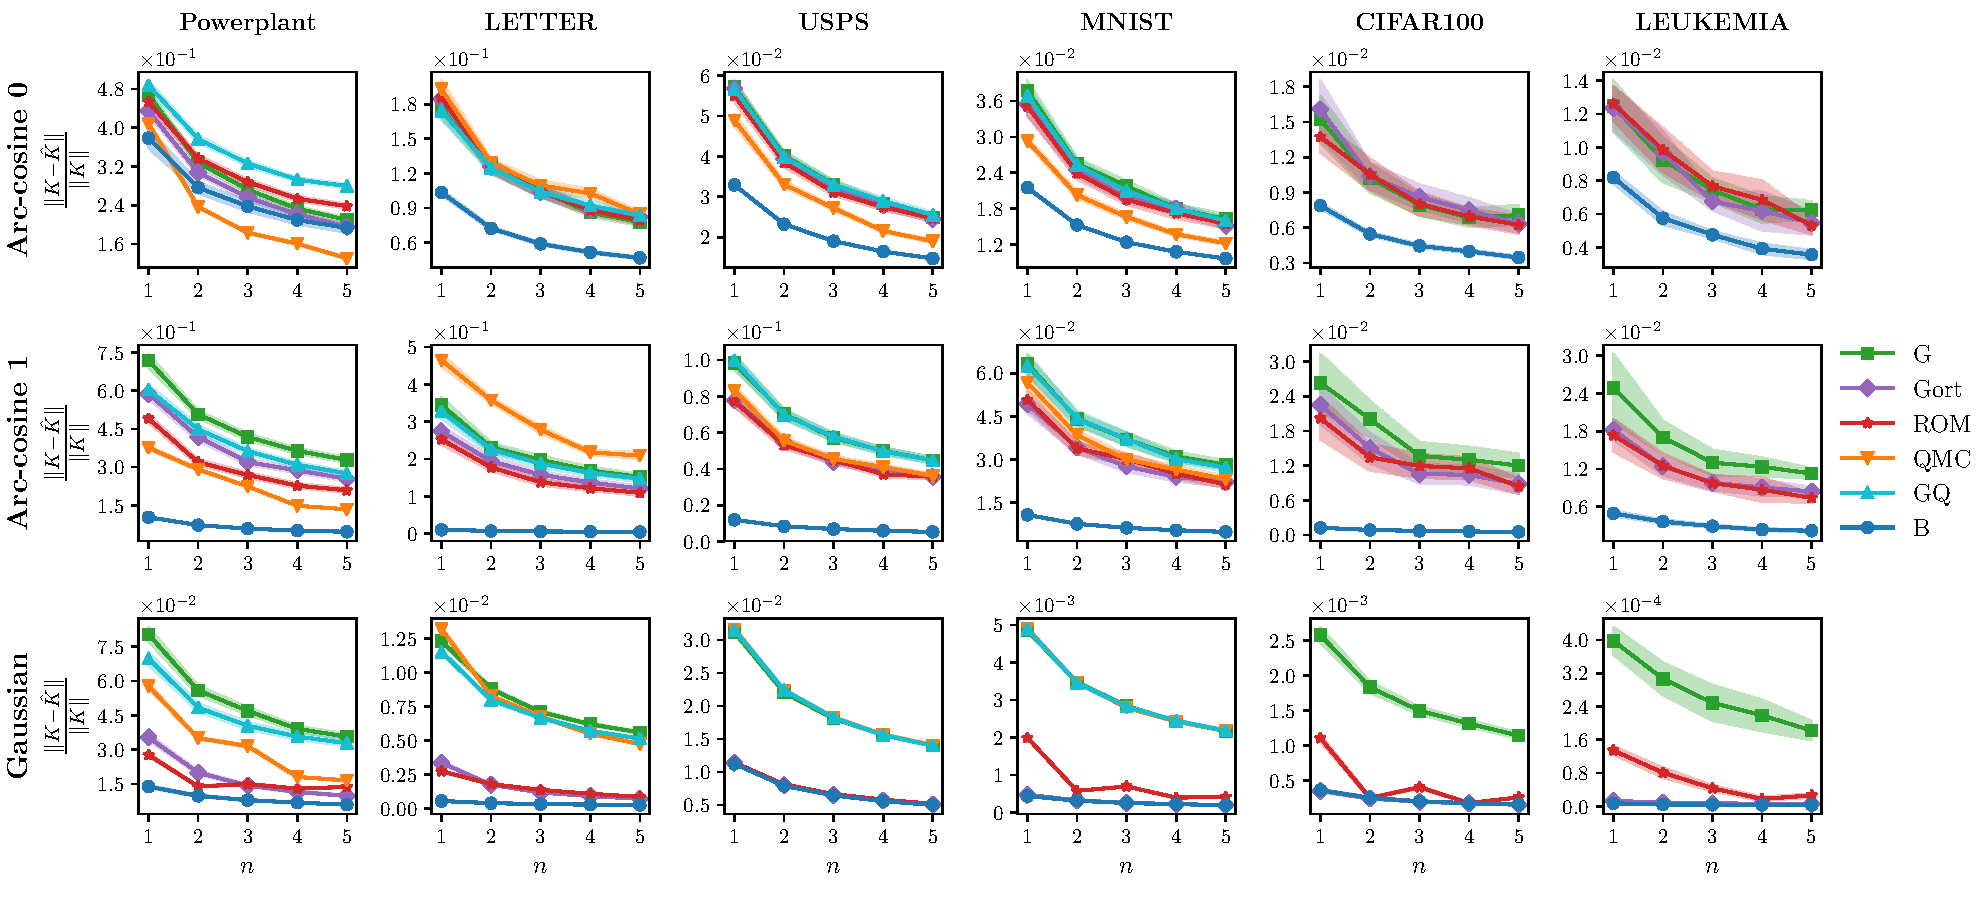
\includegraphics[width=\textwidth]{figures/quadratures/kernel_acc}
\caption{Kernel approximation error across three kernels and 6 datasets.Lower is better. The x-axis represents the factor to which we extend the original feature space, $n = \frac{D}{2(d+1)+1}$, where $d$ is the dimensionality of the original feature space, $D$ is the dimensionality of the new feature space.}
\label{fig:KA}
\end{figure*}
To measure kernel approximation quality we use relative error in Frobenius norm
$\frac{\Vert \mathbf{K} - \mathbf{\hat{K}}\Vert_{F}}{\Vert \mathbf{K} \Vert_{F}}$,
where $\mathbf{K}$ and $\mathbf{\hat{K}}$ denote exact kernel matrix and its approximation.
In line with other works we run experiments for the kernel approximation on a random
subset of a dataset.
Table \ref{table:experimental_setting} displays the settings for the experiments across the
datasets.
\begin{table}[h]
    \centering
    \caption{Space and time complexity.}
    \label{table:complexity}
    \begin{tabular}{ c  c  c }
    \textbf{Method} & \textbf{Space} & \textbf{Time} \\
    \hline
    ORF & $\mathcal{O}(Dd)$ & $\mathcal{O}(Dd)$ \\
    QMC & $\mathcal{O}(Dd)$ & $\mathcal{O}(Dd)$ \\
    ROM & $\mathcal{O}(d)$ & $\mathcal{O}(d\log d)$ \\
    \textbf{Quadrature based} & $\mathcal{O}(d)$ & $\mathcal{O}(d\log d)$ \\
    \hline
    \end{tabular}
\end{table}
\begin{table}[h]
    \centering
    \caption{Experimental settings for the datasets.}
    \label{table:experimental_setting}
    \begin{tabular}{ c c c c c }
    \textbf{Dataset} & $N$ & $d$ & \textbf{\#samples} & \textbf{\#runs} \\
    \hline
    Powerplant & 9568 & 4 & 550 & 500 \\
    LETTER & 20000 & 16 & 550 & 500 \\
    USPS & 9298 & 256 & 550 & 500 \\
    MNIST & 70000 & 784 & 550 & 100 \\
    CIFAR100 & 60000 & 3072 & 50 & 50 \\
    LEUKEMIA & 72 & 7129 & 10 & 10 \\
    \hline
    \end{tabular}
\end{table}

Approximation was constructed for different number of $SR$ samples $n = \frac{D}{2(d+1)+1}$,
where $d$ is an original feature space dimensionality and $D$ is the new one. For the Gaussian
kernel we set hyperparameter $\gamma = \frac{1}{2\sigma^2}$ to the default value of
$\frac{1}{d}$ for all the approximants, while the arc-cosine kernels (see definition of
arc-cosine kernel in the Appendix) have no hyperparameters.

We run experiments for each [kernel, dataset, $n$] tuple and plot 95\% confidence interval around the mean value line. Figure \ref{fig:KA} shows the results for kernel approximation error on LETTER, MNIST, CIFAR100 and LEUKEMIA datasets.

QMC method almost always coincides with RFF except for arc-cosine 0 kernel. It particularly enjoys Powerplant dataset with $d=4$, i.e. small number of features. Possible explanation for such behaviour can be due to the connection with QMC quadratures. The worst case error for QMC quadratures scales with $n^{-1}(\log n)^d$, where $d$ is the dimensionality and $n$ is the number of sample points \citep{owen1998latin}. It is worth mentioning that for large $d$ it is also a problem to construct a proper QMC point set. Thus, in higher dimensions QMC may bring little practical advantage over MC. While recent randomized QMC techniques indeed in some cases have no dependence on $d$, our approach is still computationally more efficient thanks to the structured matrices. GQ method as well matches the performance of RFF. We omit both QMC and GQ from experiments on datasets with large $d = [3072, 7129]$ (CIFAR100, LEUKEMIA).

The empirical results in Figure \ref{fig:KA} support our hypothesis about the advantages of $\mathbf{SR}$ quadratures applied to kernel approximation compared to SOTA methods.
With an exception of a couple of cases: (Arc-cosine 0, Powerplant) and (Gaussian, USPS), our method displays clear exceeding performance.

\subsection{Classification/regression with new features}
\label{sub:finalscore}
\begin{figure*}[h]
\centering
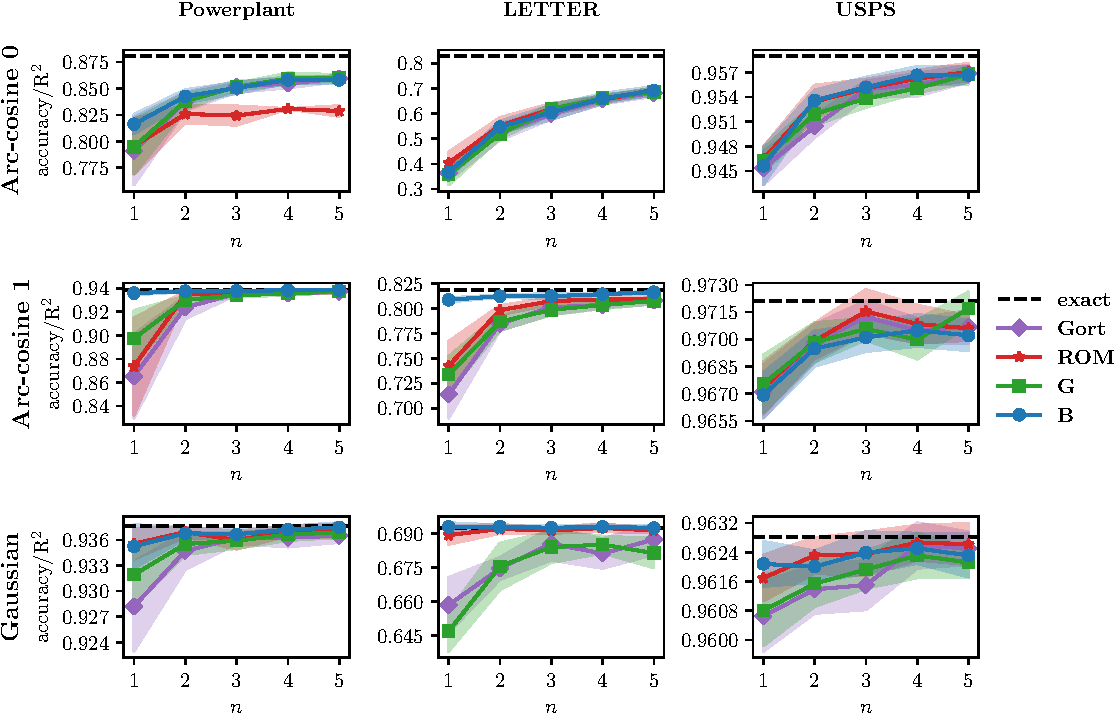
\includegraphics[width=0.8\textwidth]{figures/quadratures/Powerplant_LETTER_USPSacc_plain}
\caption{Accuracy/$R^2$ score using embeddings with three kernels on 3 datasets. Higher is better.
The x-axis represents the factor to which we extend the original feature space, $n = \frac{D}{2(d+1)+1}$.}
\label{fig:acc}
\end{figure*}

We estimate accuracy and $R^2$ scores for the classification/regression tasks on some of the datasets (Figure~\ref{fig:acc}).
We examine the performance with the same setting as in experiments for kernel approximation error, except now we map the whole dataset.
We use Support Vector Machines to obtain predictions.

Kernel approximation error does not fully define the final prediction accuracy -- the best performing kernel matrix approximant not necessarily yields the best accuracy or $R^2$ score. However, the empirical results illustrate that our method delivers comparable and often superior quality on the downstream tasks.

\subsection{Walltime experiment}
We measure time spent on explicit mapping of features by running each experiment 50 times and averaging the measurements.  Indeed, Figure \ref{fig:walltime} demonstrates that the method scales as theoretically predicted with larger dimensions thanks to the structured nature of the mapping.

\begin{figure}[h]
\centering
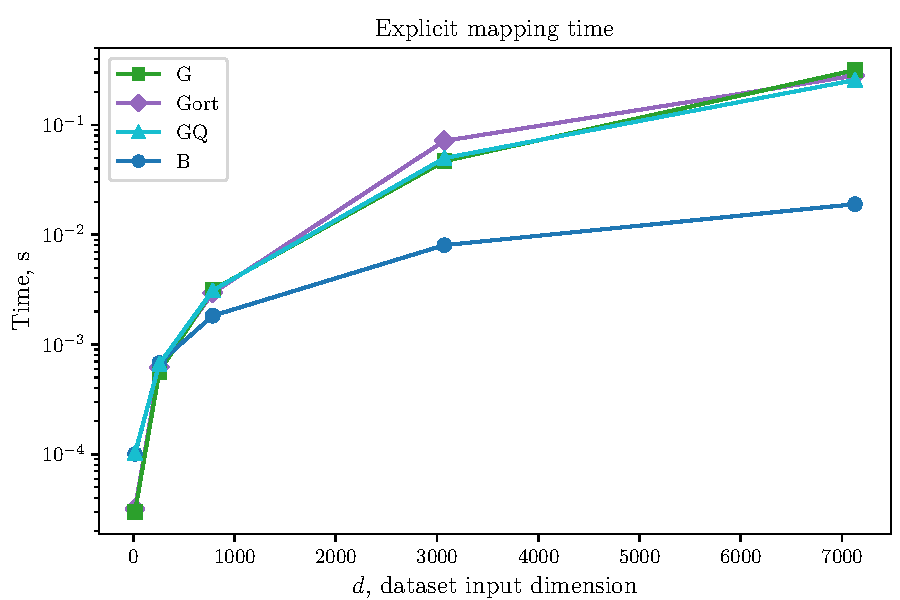
\includegraphics[width=0.4\textwidth]{figures/quadratures/time_r}
\caption{Time spent on explicit mapping. The x-axis represents the 5 datasets with increasing input number of features: LETTER, USPS, MNIST, CIFAR100 and LEUKEMIA.}
\label{fig:walltime}
\end{figure}

\section{Related work}
\label{sec:related_work}
In this section we provide brief review of the existing approaches
connected to the low-rank approximation of the kernel function.

The most popular methods for scaling up kernel methods are based on a low-rank approximation of the kernel using either data-dependent or independent basis functions.
The first one includes Nystr{\" o}m method \citep{drineas2005nystrom}, greedy basis selection techniques \citep{smola2000sparse}, incomplete Cholesky decomposition \citep{fine2001efficient}.

The construction of basis functions in these techniques utilizes the given training set making them more attractive for some problems compared to Random Fourier Features approach.
In general, data-dependent approaches perform better than data-independent approaches when there is a gap in the eigen-spectrum of the kernel matrix.
The rigorous study of generalization performance of both approaches can be found in \citep{yang2012nystrom}.

In data-independent techniques, the kernel function is approximated directly.
Most of the methods (including the proposed approach) that follow this idea are based on Random Fourier Features \citep{rahimi2008random}. They require so-called weight matrix that can be generated in a number of ways.
\citep{le2013fastfood} form the weight matrix as a product of
structured matrices.
It enables fast computation of matrix-vector products and speeds up generation of random features.

Another work \citep{felix2016orthogonal} orthogonalizes the features by means of orthogonal weight matrix.
This leads to less correlated and more informative features increasing the quality of approximation. They support this result both analytically and empirically.
The authors also introduce matrices with some special structure for fast computations.
\citep{choromanski2017unreasonable} propose a generalization of the ideas from \citep{le2013fastfood} and \citep{felix2016orthogonal}, delivering an analytical estimate for the mean squared error (MSE) of approximation.

All these works use simple Monte Carlo sampling.
However, the convergence can be improved by changing Monte Carlo sampling to Quasi-Monte Carlo sampling.
Following this idea \citep{yang2014quasi} apply quasi-Monte Carlo to Random Fourier Features.
In \citep{yu2015compact} the authors make attempt to improve quality of the approximation of Random Fourier Features by optimizing sequences conditioning on a given dataset.

Among the recent papers there are works that, similar to our approach, use the numerical integration methods to approximate kernels. While \citep{bach2017equivalence} carefully inspects the connection between random features and quadratures, they did not provide any practically useful explicit mappings for kernels. Leveraging the connection \citep{dao2017gaussian} propose several methods with Gaussian quadratures. Among them three schemes are data-independent and one is data-dependent. The authors do not compare them with the approaches for random feature generation other than random Fourier features. The data-dependent scheme optimizes the weights for the quadrature points to yield better performance.